% !TeX spellcheck = es_CO
\documentclass[oneside]{book}
\usepackage{braket}
\usepackage[latin1]{inputenc}
\usepackage{amsfonts}
\usepackage{amsthm}
\usepackage{amsmath}
\usepackage{mathrsfs}
%\usepackage{empheq}
\usepackage{enumitem}
\usepackage[pdftex]{color,graphicx}
\usepackage{hyperref}
\usepackage{listings}
\usepackage{calligra}
\usepackage{algpseudocode} 
\DeclareFontShape{T1}{calligra}{m}{n}{<->s*[2.2]callig15}{}
\newcommand{\scripty}[1]{\ensuremath{\mathcalligra{#1}}}
\setlength{\oddsidemargin}{0cm}
\setlength{\textwidth}{490pt}
\setlength{\topmargin}{-40pt}
\addtolength{\hoffset}{-0.3cm}
\addtolength{\textheight}{4cm}
\usepackage{amssymb}
\usepackage{graphicx} % Required for the inclusion of images
\setlength\parindent{0pt} % Removes all indentation from paragraphs
\usepackage{float}
\usepackage{makeidx}

%\begin{figure}[H]
%	\centering
%	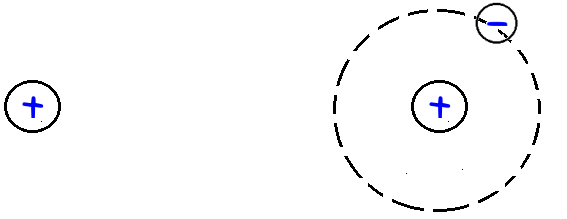
\includegraphics[scale = 0.42]{lcaoderecha}
%	\caption{Eletr\'on ligado solo al n�cleo derecho}
%	\label{fig1}
%	\end{figure}




\begin{document}

\begin{center}
\textsc{\LARGE Mec�nica Cu�ntica II}\\[0.5cm]
\textsc{\LARGE Colisiones Elasticas Sin Creaci�n Ni Aniquilaci�n de Part�culas}\\[0.5cm]
\end{center}


\begin{center}
\begin{tabular}{l r}
\large
Notas de clase del Profesor: Luis Quiroga Puello% Instructor/supervisor
\normalsize
\end{tabular}
\end{center}

\textbf{\large Estas son las notas de clase tomadas en el semestre 20151 en la clase Mec\'anica Cu\'antica II dictada por el profesor Luis Quiroga en La Universidad de los Andes. Estas notas son escritas por un alumno y pueden contener errores, uselas con precauci\'on.}


\tableofcontents

\pagebreak






\chapter{Suma de Momentos Angulares}

\begin{equation}
\label{1}  \widehat{J}_1^2 \ket{j_1,j_2,m_1,m_2} = \hbar^2 j_1(j_1+1)\ket{j_1,j_2,m_1,m_2}
\end{equation}


\begin{equation}
\label{2}  \widehat{J}_{z_1} \ket{j_1,j_2,m_1,m_2} = \hbar\; m_1\ket{j_1,j_2,m_1,m_2}
\end{equation}


\begin{equation}
\label{3}  \widehat{J}_2^2 \ket{j_1,j_2,m_1,m_2} = \hbar^2 j_2(j_2+1)\ket{j_1,j_2,m_1,m_2}
\end{equation}


\begin{equation}
\label{4}  \widehat{J}_{z_2} \ket{j_1,j_2,m_1,m_2} = \hbar\; m_2\ket{j_1,j_2,m_1,m_2}
\end{equation}


Considere dos momentos angulares arbitrarios $\widehat{J}_1$ y $\widehat{J}_2$. En la base con informaci�n individual de cada momento angular se tiene los estados propios que act�an como se muestra en las relaciones (\ref{1} -  \ref{4}).

\begin{equation}
	\label{5}  \widehat{J}_T = \widehat{J}_1 + \widehat{J}_2
\end{equation}


\begin{equation}
	\label{6}  \widehat{J}_T^2 \color{blue} \ket{j_1,j_2,J,M}\color{black}= \hbar^2 J(J+1) \color{blue}\ket{j_1,j_2,J,M}  \color{black}
\end{equation}


\begin{equation}
\label{7}  \widehat{J}_{z_T} \color{blue}\ket{j_1,j_2,J,M}\color{black}= \hbar\; M \color{blue}\ket{j_1,j_2,J,M}  \color{black}
\end{equation}


Se define el operador de momento angular $\widehat{J}_T$ como se muestra en (\ref{5}). En la base colectiva(en azul) que es la base de vectores propios del operador de momento angular total y momento angular total en la direcci�n $z$, se cumplen las relaciones (\ref{6} - \ref{7}). Se desea conocer los valores propio de los operadores totales y como escribir la base colectiva como combinaci�n lineal de la base individual.


\begin{equation}
\label{8}  M_{\text{max}} = j_1 + j_2  
\end{equation}


\begin{equation}
\label{9}  |j_1 - j_2| \leq J \leq j_1 + j_2 
\end{equation}


\begin{equation}
\label{10}  M \in \left\{ -(j_1 + j_2 ), -(j_1 + j_2 -1), \dots ,0,\dots,(j_1 + j_2 -1), j_1 + j_2  \right\}  
\end{equation}


\begin{equation}
\label{11}  J \in \left\{0 \text{ � } 1/2  ,\dots, j_1 + j_2-1, j_1 + j_2  \right\}  
\end{equation}

Los valores propios de   $\widehat{J}_T$ y $\widehat{J}_{z_T}$ estan dados por (\ref{10} - \ref{11}), que son una consecuencia directa de (\ref{8} - \ref{9}) por teor�a del momento angular.
  



\begin{equation}
\label{12}    \widehat{J}_{z_T} \ket{j_1,j_2,m_1,m_2}= \hbar(m_1+m_2) \ket{j_1,j_2,m_1,m_2} 
\end{equation}



\begin{equation}
\label{16}     \color{blue}\ket{j_1,j_2,j_1+j_2,j_1+j_2} \color{black}=  \ket{j_1,j_2,j_1,j_2} 
\end{equation}



De (\ref{12}) se observa que el vector propio del m�ximo valor $m_1+m_2$ ya es vector propio de la base colectiva, con $M=j_1+j_2$. De este vector propio se puede construir el resto de vectores propios con el mismo momento angular total por medio del operador escalera.


\begin{equation}
\label{13}    \widehat{J}^{\pm} =  \widehat{J}^{\pm}_1 + \widehat{J}^{\pm}_2 
\end{equation}

\begin{equation}
\label{14}    \widehat{J}^{\pm} \color{blue}\ket{j_1,j_2,J,M}\color{black} = \hbar \sqrt{J(J+1)-M(M\pm 1)}\color{blue}\ket{j_1,j_2,J,M\pm 1} \color{black}
\end{equation}

\begin{equation}
\label{15}    \widehat{J}^{-} \color{blue}\ket{j_1,j_2,j_1+j_2,j_1+j_2}\color{black} = \hbar \sqrt{2(j_1+j_2)}\color{blue}\ket{j_1,j_2,j_1+j_2,j_1+j_2-1} \color{black}
\end{equation}




\begin{equation}
\label{17}    \widehat{J}^{-}\color{blue} \ket{j_1,j_2,j_1+j_2,j_1+j_2}\color{black} = (\widehat{J}^{\pm}_1 + \widehat{J}^{\pm}_2 )  \ket{j_1,j_2,j_1,j_2} = \hbar \sqrt{2j_1}\ket{j_1,j_2,j_1-1,j_2} + \hbar \sqrt{2j_2}\ket{j_1,j_2,j_1,j_2-1}
\end{equation}

Los operadores escalera se definen en (\ref{13} - \ref{15}). En la linea (\ref{15}) se aplica la definici�n para la base colectiva. En la l�nea (\ref{17}) se utiliza la representaci�n en la base individual del vector propio de la base colectiva que se conoce $M=j_1 + j_2$ y se actu� el operador escalera sobre �l. 

\begin{equation}
\label{18}   \color{blue}\ket{j_1,j_2,j_1+j_2,j_1+j_2-1}\color{black} =  \sqrt{\frac{j_1}{j_1 + j_2}}\ket{j_1,j_2,j_1-1,j_2} + \hbar \sqrt{\frac{j_2}{j_1+j_2}}\ket{j_1,j_2,j_1,j_2-1}
\end{equation}


Aplicando el operador escalera varias veces se puede obtener todos los vectores propios de $J=j_1+j_2$. Para $J=j_1+j_2-1$ se sabe lo siguiente:


\begin{equation}
\label{19}   \color{blue}\ket{j_1,j_2,j_1+j_2-1,j_1+j_2-1}\color{black} =  \alpha\ket{j_1,j_2,j_1-1,j_2} + 
\beta\ket{j_1,j_2,j_1,j_2-1}
\end{equation}

Para determinar los coeficientes $\alpha$ y $\beta$ se observa que este debe ser ortogonal a cualquier vector del subespacio con con $J=j_1+j_2$ y en particular con el que tiene $M=j_1+j_2-1$. Aprovechando esto sigue que:


\begin{equation}
\label{20}   \color{blue}\braket{j_1,j_2,j_1+j_2-1,j_1+j_2-1|j_1,j_2,j_1+j_2-,j_1+j_2-1}\color{black} = 0
\end{equation}


\begin{equation}
\label{21}  \alpha \sqrt{\frac{j_1}{j_1 + j_2}} + \beta\sqrt{\frac{j_2}{j_1 + j_2}} = 0
\end{equation}

\begin{equation}
\label{22}  \alpha^2  + \beta^2 = 1
\end{equation}

No se pierde informaci�n exigiendo que los coeficientes $\alpha$ y $\beta$ sean reales. Con exigir esto y la condici�n de normalizaci�n se puede obtener los valores de $\alpha$ y $\beta$. Conociendo este vector se puede usar nuevamente el operador escalera para obtener el resto de vectores del subespacio con $J =j_1+j_2-1$. El resto de subespacios se obtienen de forma an�loga. Los valores de los coeficientes que acompa�an la base individual al expresar la base colectiva como combinaci�n lineal de ellos se les conoce como los coeficientes de Clebsch Gordan.


\begin{equation}
\label{23} \textbf{Si  } m_1 + m_2 \neq M \longrightarrow \textbf{Coeficiente}= 0
\end{equation}

La relaci�n (\ref{23}) permite saber sin hacer c�lculos si un coeficiente de Clebsch Gordan va a ser nulo. Si un vector de la base individual tiene n�meros $m_1$ y $m_2$ que no suman el valor de $M$ inmediatamente se sabe que el coeficiente de Clebsch Gordan de ese ket es 0.



\section{Ejemplo: $J_1 = J_2 = 1/2$}


\begin{equation}
\label{1.1} \color{blue} \ket{1/2,1/2,1,1} \color{black} = \ket{1/2,1/2,1/2,1/2} 
\end{equation}


Se comienza con el m�ximo valor de $M$ que para este caso es $M=1$. 

\begin{equation}
\label{1.2} \widehat{J}^- \color{blue} \ket{1/2,1/2,1,1} \color{black} = \hbar \sqrt{2}\color{blue} \ket{1/2,1/2,1,0}
\end{equation}


\begin{equation}
\label{1.3} \widehat{J}^- \color{blue} \ket{1/2,1/2,1,1} \color{black} = J^- \ket{1/2,1/2,1/2,1/2} = \hbar \ket{1/2,1/2,-1/2,1/2} + \hbar\ket{1/2,1/2,1/2,-1/2}
\end{equation}

Aplicando el operador escalera sobre las expresiones en representaci�n individual y colectiva se obtiene las relaciones (\ref{1.2}) y (\ref{1.3}).

\begin{equation}
\label{1.4}  \color{blue} \ket{1/2,1/2,1,0} \color{black} = \frac{\hbar}{\sqrt{2}} \left[ \;\ket{1/2,1/2,-1/2,1/2} + \ket{1/2,1/2,1/2,-1/2}\;\right]
\end{equation}

Despejando se obtiene el ket $\color{blue} \ket{1/2,1/2,1,0} \color{black}$ en (\ref{1.4}).

\begin{equation}
\label{1.5}  \color{blue} \ket{1/2,1/2,1,-1} \color{black} = \ket{1/2,1/2,-1/2,-1/2}
\end{equation}


\section{Ejemplo: $J_1 = J_2 = 1$}

\end{document}